% -----------------------------------------------------------------------------
% Copyright &copy; 2015 Ben Blazak <bblazak@fullerton.edu>  
% This work is licensed under a [Creative Commons Attribution 4.0 International
% License] (http://creativecommons.org/licenses/by/4.0/)  
% -----------------------------------------------------------------------------

% -----------------------------------------------------------------------------
% Copyright &copy; 2015 Ben Blazak <bblazak@fullerton.edu>  
% This work is licensed under a [Creative Commons Attribution 4.0 International
% License] (http://creativecommons.org/licenses/by/4.0/)  
% -----------------------------------------------------------------------------

% - [Which lua environment should I use?] (http://tex.stackexchange.com/a/33102)
\directlua{require('scripts/functions.lua')}

\ifx\question\undefined
  \long\def \question #1{#1}
\fi
\ifx\answer\undefined
  \long\def \answer #1{#1}
\fi

% -----------------------------------------------------------------------------

\def \docTitle  {\directlua{tex.print(doc_title('\jobname'))}}
\def \docAuthor {\question{Name:\hfill{}CWID:\hfill}\answer{Answer Key}}
\def \docClass  {CPSC 121-11}
\def \docSchool {~}
\def \docTerm   {CSUF Fall 2015}

\def \docCopyright {
  \begin{figure}[b!]
    \tiny
    {\answer{\color{red}}\question{\color{.}}\hrule}
    \vspace{2ex}
    \begin{minipage}[c]{0.10\textwidth} \vspace{0ex} \vspace{-1pt}
      
\includegraphics[height=5ex]{images/ccby}
    \end{minipage}
    \begin{minipage}[c]{0.90\textwidth} \vspace{0ex}
      Copyright \copyright{} Ben Blazak \url{bblazak@fullerton.edu}\\
      This work is licensed under a Creative Commons Attribution 4.0
      International License \url{http://creativecommons.org/licenses/by/4.0/}
    \end{minipage}
    \vspace{-.14in}
    \vspace{2ex}
  \end{figure}
}

% -----------------------------------------------------------------------------

\documentclass{article}

\usepackage[includehead,
%             includefoot,
            margin=1in,
            top=.25in,
            headheight=.75in,
            headsep=.25in,
            footskip=.25in,
           ]{geometry}

\usepackage[export]{adjustbox}
\usepackage[fleqn]{amsmath}
\usepackage{amssymb}
\usepackage[shortlabels]{enumitem}
\usepackage{etoolbox}
\usepackage{fancyhdr}
\usepackage{lastpage}
\usepackage[cachedir={.minted-\jobname}]{minted}
\usepackage{tcolorbox}
\usepackage{tikz}
\usepackage[explicit]{titlesec}

\usepackage[T1]{fontenc}
\usepackage[utf8]{inputenc}
\usepackage{lmodern}

\usepackage{xcolor}

% - [Illegal parameter number in definition of \Hy@tempa]
%   (https://kba49.wordpress.com/2013/04/12/illegal-parameter-number-in-definition-of-hytempa/)
\usepackage{hyperref}

% text ------------------------------------------------------------------------

\binoppenalty = 10000  % never break next to a binary operator
\relpenalty   = 10000  % never break next to a relation operator

\setlength{\parindent}{0em}
\setlength{\parskip}{1ex}

\setlist[itemize]{nosep,itemsep=.5ex,parsep=.5ex}

% sections --------------------------------------------------------------------

% - <http://tex.stackexchange.com/a/58299>
\titleformat{name=\section}[block]{\normalfont\Large\bfseries}{}{0em}{#1\ \thesection}
% - <http://tex.stackexchange.com/a/102120>
\titleformat{name=\section,numberless}[block]{\normalfont\Large\bfseries}{}{0em}{#1}

% math ------------------------------------------------------------------------

\setlength{\mathindent}{1cm}

% - "\begin{document}" resets these values, so they have to be treated
%   specially
\AtBeginDocument{
  \setlength{\abovedisplayskip}{1.5ex plus .5ex minus .5ex}
  \setlength{\belowdisplayskip}{1.5ex plus .5ex minus .5ex}
}

% source code -----------------------------------------------------------------

\usemintedstyle{solarizedlight}
\setminted{frame=single}

\fvset{samepage=true}

% header and footer -----------------------------------------------------------

\pagestyle{fancy}

\renewcommand{\headrule}{{\answer{\color{red}}\question{\color{.}}
                          \vskip 0.5ex \hrule height 0.4pt \vskip 0.5ex}}
\renewcommand{\footrule}{{\answer{\color{red}}\question{\color{.}}
                          \vskip 0.5ex \hrule height 0.4pt \vskip 0.5ex}}

\fancyhead[L]{{\answer{\color{red}}\question{\color{.}}\docAuthor}
              {\color{.}\\\docClass}}
\fancyhead[C]{{\color{.}\docSchool\\}}
\fancyhead[R]{{\color{.}\docTerm\\\docTitle}}

\fancyfoot[C]{\thepage{} of \pageref{LastPage}}

% -----------------------------------------------------------------------------
% macros
% -----------------------------------------------------------------------------

% abbreviations ---------------------------------------------------------------

\def \<{\langle}
\def \>{\rangle}

\def \ε{\varepisilon}
\def \θ{\vartheta}
\def \κ{\varkappa}
\def \π{\varpi}
\def \ρ{\varrho}
\def \σ{\varsigma}
\def \φ{\varphi}

\def \Γ{\varGamma}
\def \Δ{\varDelta}
\def \Θ{\varTheta}
\def \Λ{\varLambda}
\def \Ξ{\varXi}
\def \Π{\varPi}
\def \Σ{\varSigma}
\def \Υ{\varUpsilon}
\def \Φ{\varPhi}
\def \Ψ{\varPsi}
\def \Ω{\varOmega}

% special characters ----------------------------------------------------------

\catcode `α = \active \let α \alpha
\catcode `β = \active \let β \beta
\catcode `γ = \active \let γ \gamma
\catcode `δ = \active \let δ \delta
\catcode `ε = \active \let ε \epsilon
\catcode `ζ = \active \let ζ \zeta
\catcode `η = \active \let η \eta
\catcode `θ = \active \let θ \theta
\catcode `ι = \active \let ι \iota
\catcode `κ = \active \let κ \kappa
\catcode `λ = \active \let λ \lambda
\catcode `μ = \active \let μ \mu
\catcode `ν = \active \let ν \nu
\catcode `ξ = \active \let ξ \xi
\catcode `ο = \active \let ο o
\catcode `π = \active \let π \pi
\catcode `ρ = \active \let ρ \rho
\catcode `σ = \active \let σ \sigma
\catcode `τ = \active \let τ \tau
\catcode `υ = \active \let υ \upsilon
\catcode `φ = \active \let φ \phi
\catcode `χ = \active \let χ \chi
\catcode `ψ = \active \let ψ \psi
\catcode `ω = \active \let ω \omega

\catcode `Α = \active \let Α A
\catcode `Β = \active \let Β B
\catcode `Γ = \active \let Γ \Gamma
\catcode `Δ = \active \let Δ \Delta
\catcode `Ε = \active \let Ε E
\catcode `Ζ = \active \let Ζ Z
\catcode `Η = \active \let Η H
\catcode `Θ = \active \let Θ \Theta
\catcode `Ι = \active \let Ι I
\catcode `Κ = \active \let Κ K
\catcode `Λ = \active \let Λ \Lambda
\catcode `Μ = \active \let Μ M
\catcode `Ν = \active \let Ν N
\catcode `Ξ = \active \let Ξ \Xi
\catcode `Ο = \active \let Ο O
\catcode `Π = \active \let Π \Pi
\catcode `Ρ = \active \let Ρ P
\catcode `Σ = \active \let Σ \Sigma
\catcode `Τ = \active \let Τ T
\catcode `Υ = \active \let Υ \Upsilon
\catcode `Φ = \active \let Φ \Phi
\catcode `Χ = \active \let Χ X
\catcode `Ψ = \active \let Ψ \Psi
\catcode `Ω = \active \let Ω \Omega

% other -----------------------------------------------------------------------

\def \docCodeDir {./code/\directlua{tex.print(jobname_root('\jobname'))}/}
\def \docImageDir {./images/\directlua{tex.print(jobname_root('\jobname'))}/}

\long\def \textAnswer #1{\answer{{\color{red!50!black}#1}}}
\long\def \textQuestion #1{\question{{\color{.}#1}}}

\long\def \standardsSection #1{{
  \section*{Standards}
  \def\arraystretch{2}
  \setlength\tabcolsep{1em}
  \begin{tabular}{|r|l|}
    \hline \textbf{Standard} & \textbf{Score} \\\hline #1
  \end{tabular}
  \docCopyright
  \newpage
}
  \def\docCopyright{}
}
\long\def \standards #1{{
  \vspace{-1em}
  \def\arraystretch{2}
  \setlength\tabcolsep{1em}
  \begin{tabular}{|r|l|}
    \hline #1
  \end{tabular}
  \vspace{1em}
}}
\def \standard #1{
  #1 & ~~~ \\\hline
}

\def \evaluateCodeTop #1#2{
  \def\codeFile{\docCodeDir/.#1.cpp.gen.section.#2}
  \IfFileExists{\docCodeDir/.#1.gen.output.gen.section.#2}
               {\def\outputFile{\docCodeDir/.#1.gen.output.gen.section.#2}}
               {\def\outputFile{\docCodeDir/.#1.gen.output.gen.section.all}}
  \par
  \inputminted{cpp}{\codeFile}
  \textQuestion{
    \inputminted[label={\normalsize{}Output},fontsize=\Large]{text}
      {\outputFile.gen.blank}
  }
  \textAnswer{
    \inputminted[label={\normalsize{}Output},fontsize=\Large]{text}
      {\outputFile}
  }
  \par
}
\def \evaluateCodeLeft #1#2{
  \def\codeFile{\docCodeDir/.#1.cpp.gen.section.#2}
  \IfFileExists{\docCodeDir/.#1.gen.output.gen.section.#2}
               {\def\outputFile{\docCodeDir/.#1.gen.output.gen.section.#2}}
               {\def\outputFile{\docCodeDir/.#1.gen.output.gen.section.all}}
  \par
  \begin{minipage}[t]{0.5\linewidth} \vspace{0ex}
    \inputminted{cpp}{\codeFile}
  \end{minipage}
  \begin{minipage}[t]{0.5\linewidth} \vspace{0ex}
    \textQuestion{
      \inputminted[label=Output]{text}{\codeFile.gen.blank}
    }
    \textAnswer{
      \inputminted[label=Output]{text}{\outputFile}
    }
  \end{minipage}
  \par
}

\def \showCodeTop #1#2{
  \def\codeFile{\docCodeDir/.#1.cpp.gen.section.#2}
  \IfFileExists{\docCodeDir/.#1.gen.output.gen.section.#2}
               {\def\outputFile{\docCodeDir/.#1.gen.output.gen.section.#2}}
               {\def\outputFile{\docCodeDir/.#1.gen.output.gen.section.all}}
  \par
  \inputminted{cpp}{\codeFile}
  \vspace{0.5\parskip}
  \inputminted[label=Output]{text}{\outputFile}
  \par
}
\def \showCodeLeft #1#2{
  \def\codeFile{\docCodeDir/.#1.cpp.gen.section.#2}
  \IfFileExists{\docCodeDir/.#1.gen.output.gen.section.#2}
               {\def\outputFile{\docCodeDir/.#1.gen.output.gen.section.#2}}
               {\def\outputFile{\docCodeDir/.#1.gen.output.gen.section.all}}
  \par
  \begin{minipage}[t]{0.5\linewidth} \vspace{0ex}
    \inputminted{cpp}{\codeFile}
  \end{minipage}
  \begin{minipage}[t]{0.5\linewidth} \vspace{0ex}
    \inputminted[label=Output]{text}{\outputFile}
  \end{minipage}
  \par
}



\def \memoryImage{%
  \par\medskip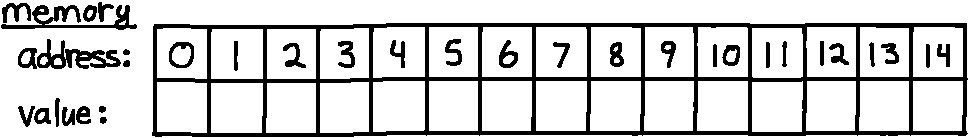
\includegraphics[width=\linewidth,valign=t]{\docImageDir/memory}%
}

\def \code #1{{
  \inputminted{cpp}{\docCodeDir/.#1.cpp.gen.section.array}
}}

% -----------------------------------------------------------------------------

\begin{document}
\docCopyright

\section*{Instructions}

For questions with a picture illustrating memory, assume that the memory slots
are one \mintinline{cpp}{int} wide, and use ``?'' in a slot to indicate that it
contains an undefined value.  For each array, label an appropriately sized
group of slots with the array name, and fill in the slots with the array's
values.

\subsection*{Example}
\vspace{-2ex}
\begin{minipage}[t]{0.5\linewidth} \vspace{0ex}
  \vspace{-2.7ex}
  \memoryImage
  \par
  \vspace{-0.63in}
  \hspace{0.45in}
  
\includegraphics[width=1.15in]{\docImageDir/example}
\end{minipage}
\begin{minipage}[t]{0.5\linewidth} \vspace{0ex}
  \code{example}
\end{minipage}

\section{Question}
\standards{
  \standard{arrays}
}

\begin{itemize}

  \item What is the index of the first element of an array?
    \textAnswer{\par
      Answer: \mintinline{cpp}{0}
    }
    \vfill

  \item What is the index of the last element of any array that holds 5 values?
    \textAnswer{\par
      Answer: \mintinline{cpp}{4}
    }
    \vfill

  \item What happens when you access an element of the array that does not
    exist?
    \textAnswer{\par
      If the program is allowed to access the location in memory then that
      location in memory is accessed as if it were an element of the array
      (regardless of what's actually there).  If the program doesn't have
      access to the location in memory, a segmentation fault (segfault) will
      occur, and the operating system will kill the process.
    }
    \vfill
    \vfill

  \item \memoryImage
    \textAnswer{\par
      \par
      \vspace{-1.14in}
      \hspace{0.9in}
      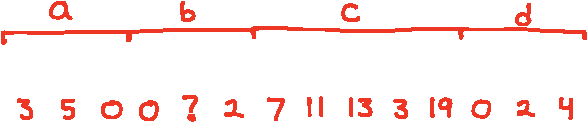
\includegraphics[width=4.87in]{\docImageDir/question}
    }
    \code{question}

\end{itemize}

\end{document}

